\ifdefined\standalone
\documentclass[12pt]{article}
\usepackage{graphicx}
\usepackage{float}
\usepackage[a4paper, margin=1in]{geometry}
\usepackage{amsmath}
\usepackage{tikz}
\usetikzlibrary{decorations.pathmorphing}
\usepackage[hidelinks]{hyperref}

\begin{document}
\fi


\section{3D Cone Calorimeter with Lateral Convection}

This case extends the reference cone calorimeter configuration into three dimensions by introducing natural convection on the lateral $x$ and $y$ surfaces, in addition to the top-applied heat flux. This setup induces multidimensional effects in the degradation front propagation, resulting in a more realistic physical behavior.

The domain consists of a 6~cm thick slab of \textbf{Material A} atop a 12~cm Kaowool insulation layer, with lateral dimensions of 10~cm $\times$ 10~cm. A vertical mid-plane at $x = 5$~cm (shown in gray in Figure~\ref{fig:3d_config}) is used to visualize the pyrolysis front using Smokeview. Figure~\ref{fig:reaction_rate_evolution} shows the reaction rate distribution in this plane at various time steps.

The computational grid uses uniform spacing: $\Delta z = 0.1$~mm to resolve vertical gradients, and $\Delta x = \Delta y = 5$~mm laterally. A fixed time step of $\Delta t = 0.5$~s is applied. The solver is configured with \texttt{SOLVE\_MAIN\_DIRECTIONS = Z}.

\vspace{1em}

\begin{figure}[H]
\centering
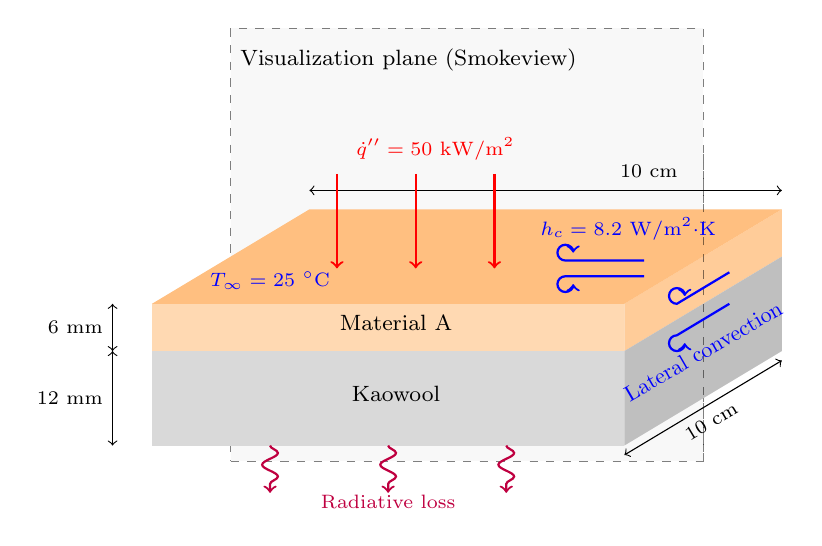
\begin{tikzpicture}[scale=1, x={(1cm,0cm)}, y={(0cm,1cm)}, z={(0.5cm,0.3cm)}]

% Dimensions of Material A
\def\LA{6}  % length (x)
\def\WA{0.6} % width (y)
\def\HA{4}  % height (z)

% Mid-height visualization plane
\filldraw[fill=gray!10, draw=black, dashed, opacity=0.5]
  (0, -2, \HA/2) --
  (\LA, -2, \HA/2) --
  (\LA, 3.5, \HA/2) --
  (0, 3.5, \HA/2) -- cycle;

\node[anchor=west] at (0,3.1,\HA/2) {\footnotesize Visualization plane (Smokeview)};

% Material A block
\fill[orange!30] (0,0,0) -- (\LA,0,0) -- (\LA,\WA,0) -- (0,\WA,0) -- cycle;
\fill[orange!40] (\LA,0,0) -- (\LA,\WA,0) -- (\LA,\WA,\HA) -- (\LA,0,\HA) -- cycle;
\fill[orange!50] (0,\WA,0) -- (\LA,\WA,0) -- (\LA,\WA,\HA) -- (0,\WA,\HA) -- cycle;

% Kaowool insulation
\def\LK{\LA}
\def\WK{2*\WA}
\def\HK{\HA}

\fill[gray!30] (0,-\WK,0) -- (\LK,-\WK,0) -- (\LK,0,0) -- (0,0,0) -- cycle;
\fill[gray!50] (\LK,-\WK,0) -- (\LK,0,0) -- (\LK,0,\HK) -- (\LK,-\WK,\HK) -- cycle;

\draw[draw=black, dashed, opacity=0.5] (\LA,-2,\HA/2) -- (\LA,2,\HA/2);

% Labels
\node at (\LA/2,\WA/2,0.2) {\footnotesize Material A};
\node at (\LK/2,-\WK/2,0.2) {\footnotesize Kaowool};

% Annotations
\draw[<->] (-0.5,0,0) -- (-0.5,0.6,0);
\node[left] at (-0.5,0.3,0) {\scriptsize 6~mm};

\draw[<->] (-0.5,-1.2,0) -- (-0.5,0,0);
\node[left] at (-0.5,-0.6,0) {\scriptsize 12~mm};

\draw[<->] (0,1.4*\WA,\HA) -- (\LA,1.4*\WA,\HA);
\node[left] at (4*\LA/5,1.8*\WA,\HA) {\scriptsize 10~cm};

\draw[<->] (\LA,-1.1*\WK,\HA) -- (\LA,-1.1*\WK,0)
  node[midway, sloped, below] {\scriptsize 10~cm};

% Heat flux
\foreach \x in {1.8,2.8,3.8}
    \draw[->,thick,red] (\x-0.2,1.8,1.5) -- (\x-0.2,0.6,1.5);
\node[above,red] at (2.6,1.7,2) {\scriptsize $\dot{q}'' = 50~\mathrm{kW/m^2}$};

% Vertical convection
\draw[->,thick, blue] (6,0.8,0.5) -- (5,0.8,0.5) arc[start angle=90, end angle=360, radius=0.1cm]; 
\draw[->,thick, blue] (6,1,0.5) -- (5,1,0.5) arc[start angle=270, end angle=0, radius=0.1cm]; 

\node[blue] at (5.8,1.4,0.5) {\scriptsize $h_c = 8.2~\mathrm{W/m^2{\cdot}K}$};
\node[blue] at (1,0.6,1) {\scriptsize $T_\infty = 25~^\circ\mathrm{C}$};

% Lateral convection
\draw[->,thick, blue] (\LA,0.2,2*\HA/3) -- (\LA,0.2,1*\HA/3) arc[start angle=270, end angle=0, radius=0.1cm]; 
\draw[->,thick, blue] (\LA,-0.2,2*\HA/3) -- (\LA,-0.2,1*\HA/3) arc[start angle=90, end angle=360, radius=0.1cm]; 

\node[rotate=30, scale=0.8, blue] at (\LA, -\WK/2, \HA/2) {Lateral convection};

% Radiative loss
\foreach \x in {1.5,3,4.5}
    \draw[purple,thick,->,decorate,decoration={snake,amplitude=1mm,segment length=3mm}] (\x,-1.2,0) -- (\x,-1.8,0);
\node[below,purple] at (3,-1.7,0) {\scriptsize Radiative loss};

\end{tikzpicture}
\caption{Three-dimensional configuration.}
\label{fig:3d_config}
\end{figure}

\begin{figure}[H]
\centering
\includegraphics[width=0.85\linewidth]{smokeview_3D_conv.png}
\caption{Reaction rate distribution in the mid-height plane $YZ$ at different times.}
\label{fig:reaction_rate_evolution}
\end{figure}

\ifdefined\standalone
\end{document}
\fi

